%
%  Vincent Yannello
%
\documentclass[12pt,fullpage]{article}
\usepackage{fullpage}
\usepackage{psfrag}                                          % LaTeX graphics tool
\usepackage{pslatex}                                         % avoids the default cmr font
\usepackage{graphicx}                                        % graphics package 
\usepackage{epsfig}                                          % figures
\usepackage{hyperref}
\usepackage{color}

\begin{document}

\noindent
{\bf Rayleigh distribution} (from \color{blue}\url{http://www.math.wm.edu/~leemis/chart/UDR/UDR.html}\color{black})

\noindent
The shorthand $X \sim {\rm Rayleigh}(\alpha)$ is used to indicate that the
random variable $X$ has the Rayleigh distribution with parameter $\alpha$.
A Rayleigh random variable $X$ with positive parameter $\alpha$ has probability density function 
$$
f(x) = \frac{2xe^{-x^ {\kern 0.04 em 2}/\alpha}}{\alpha} \qquad \qquad x > 0.
$$
The Rayleigh distribution can be used to model the lifetime of an object or a service time.
The probability density function with three different parameter settings is illustrated below.
{\begin{figure}[h!]
\begin{center}
\psfrag{lab1}{$\alpha = 0.5$}
\psfrag{lab2}{$\alpha = 2$}
\psfrag{lab3}{$\alpha = 8$}
\psfrag{labx}{$x$}
\psfrag{labf}{$f(x)$}
\includegraphics[width=3.2in]{RayleighPlot.ps}
\end{center}
\end{figure}}\\
The cumulative distribution function on the support of $X$ is
$$
F(x) = P(X \le x) = 1 - e^{-x^ {{\kern 0.04 em 2}}/\alpha}  \qquad \qquad x > 0.
$$
The survivor function on the support of $X$ is
$$
S(x) = P(X \ge x) = e^{-x^{\kern 0.04 em 2}/\alpha}  \qquad \qquad x > 0.
$$
The hazard function on the support of $X$ is
$$
h(x) = \frac{f(x)}{S(x)} = \frac{2x}{\alpha} \qquad \qquad x > 0.
$$
The cumulative hazard function on the support of $X$ is 
$$
H(x) = - \ln S(x) = \frac{x^{\kern 0.04 em 2}}{\alpha} \qquad \qquad x>0.
$$
The inverse distribution function of $X$ is 
$$
F^{-1} (u) = \sqrt{-\alpha \ln (1 - u)} \qquad \qquad 0 < u < 1.
$$
The median of $X$ is
$$
\sqrt{\alpha \ln(2)}.
$$
The moment generating function of $X$ is mathematically intractable.
\\
\\
The characteristic function of $X$ is mathematically intractable.
\\
\\
The population mean, variance, skewness, and kurtosis of $X$ are
$$
E[X] = \frac{\sqrt{\alpha \pi}} {2} \qquad \qquad 
V[X] = \frac{\alpha(4 - \pi)} {4} \qquad \qquad 
E\left[ \left( \frac{X - \mu}{\sigma} \right) ^ {\kern -0.08 em 3} \right] = \frac{2 \sqrt{\pi} \, (\pi - 3)} {(4 - \pi) ^ {3 / 2}} \qquad \qquad 
$$
$$
E\left[ \left( \frac{X - \mu}{\sigma} \right) ^ {\kern -0.08 em 4} \right] = \frac{6 \pi (4 - \pi) - 16}{(\pi - 4) ^ 2}.
$$

\vspace{0.1in}

\noindent
{\bf APPL verification:}
The APPL statements
\begin{verbatim}
assume(alpha > 0);
X:=[[x -> (2 * x / alpha) * exp(-x ^ 2 / alpha)], [0,infinity],
    ["Continuous", "PDF"]];
CDF(X);
HF(X);
CHF(X);
Mean(X);
Variance(X);
Skewness(X);
Kurtosis(X);
\end{verbatim}
verify the cumulative distribution function, hazard function, cumulative hazard function, population mean, variance, skewness, and kurtosis.

\end{document}
